% !Mode:: "TeX:UTF-8" 

\BiChapter{绪论}{}
\BiSection{问题背景}{}
词语的相似度计算是自然语言处理中的一项基本任务。它的目的是使用自动化的方法给出一个量化的指标,来衡量一对词语之间的相似程度。词语相似度计算对于很多高层次的自然语言处理任务有着重要的意义,例如问答、信息检索、改写检测与文本蕴含。

为了评价一种词语相似度计算方法的好坏,可以使用内部任务评价或外部任务评价。内部任务评价直接使用一个标准的词语相似度标注数据集,并使用一些评价指标来衡量机器给出的结果与标准数据集之间的差异;而外部任务评价则利用词语相似度计算的结果解决其他的高层次机器学习问题,通过衡量不同计算结果在这些问题上的性能来简介衡量词语相似度计算方法的好坏。

本课题取自 NLPCC-ICCPOL 2016 会议中的“中文词语相似度计算”开放任务。该开放任务使用内部任务评价的方式来衡量各参赛队提交的结果。其组织者发布了一个 PKU-500 数据集\citeup{Wu2016},其中包含 500 个词语对,以及对每个词语对之间的相似度标注。共有 49 个参赛队伍报名参加了此次开放任务,而最终由 21 个参赛队伍提交了总计 24 个系统\citeup{Wu2016}。

\BiSection{相关工作}{}
在英文词语相似度任务中,已经有多个数据集可以作为基准测试。其中,使用最广泛的是 WordSim-353 数据集。这个数据集包含 353 个词语对,并由 16 名标注者对其相似度进行了标注。

在 NLPCC-ICCPOL 2016 会议举办之前,Semeval-2012 会议上也举行了一次中文词语相似度的比赛,比赛所使用的词语对是经过翻译的 WordSim-353 数据集,并重新进行了人工标注。遗憾的是,这次比赛只有两个队伍参加。

本次开放任务中的参赛队伍使用的方法大致分为三类:基于辞典或知识库的方法、基于语料的方法与基于信息检索的方法。

基于词典或知识库的方法利用了一些现有的语言学资源,例如知网(HowNet)和同义词词林。这些词典或知识库的作者往往同时给出了用于计算词语相似度的规则。有些参赛队伍直接使用了这些规则,还有一些对这些规则进行了修改。这些方法依赖于词典或知识库的组织结构,并且无法处理未登录词。此外,人工制定的规则是否合理也是影响模型性能的重要因素。

基于语料的方法主要是根据上下文信息进行词嵌入,这类方法假设“相似的词语应该出现在相似的上下文中”。典型的词嵌入方法,例如 word2vec,具有成熟的工具包,因此在各参赛队伍中非常受到欢迎。除了词嵌入方法以外,来自大连理工大学的参赛队\citeup{Pei2016}使用了深度学习的方法来识别描述词语类比的句子,例如“寂寞和孤单的区别是什么”。如果这类句子出现在语料中,很可能意味着这两个词语是相关的。基于语料的方法需要大规模的语料库和漫长的训练时间,由于这些模型普遍使用无需人工标注的生语料库,因此语料的获取来源非常广泛。而训练时间的缩短只能通过使用运算能力更强的硬件,因此实验可能受到硬件条件的制约。针对中文语料而言,绝大部分的模型是以词为单位进行处理,这样分词的准确度也会对模型最终性能产生一定影响。

基于信息检索的方法利用搜索引擎查询包含目标词语的页面,根据同时包含两个词语的页面数、仅包含一个词语的页面数利用公式计算目标词语的相似度。这种方法的实现非常的简单,只需爬取搜索引擎的结果页面,或调用搜索引擎提供的 API。有的队伍将这种方法作为多种评价方法之一\citeup{Ma2016},也有的队伍用信息检索得到的结果作为弱监督学习的指标\citeup{Pei2016}。这种方法的一大问题是词语相似度和词语共同出现的频率并不一致,例如一些事物的别名经常在科普类的文章中被介绍(例如“西红柿”和“番茄”),而因口语习惯而导致不同的同义词(例如“拖后腿”和“拉后腿”)就很难在一篇文章中同时出现\citeup{Zhang2017}。

\BiSection{数据生成与评价指标}{}
PKU-500 数据集的生成过程分为三个步骤,分别为词语选择、词语对生成和相似度标注。

PKU-500 数据集的词语选择过程遵循以下的条件:
\begin{enumerate}
	\item 领域:同时涉及传统书面语言与近期的网络语言。
	\item 频率:应同时包含高频、中频与低频的词语。
	\item 词性:应同时包含名词、动词与形容词。除上述实词外还应包含虚词(例如副词和连词)。
	\item 字数:应包含 1 -- 4 个字的词语。
	\item 词义:应包含部分多义词。
	\item 极性:应同时包含正面词语与负面词语。
\end{enumerate}
根据上述条件,词语的选择过程如下:
\begin{enumerate}
	\item 数据来源于两个领域:三个月的《人民日报》新闻与一大批新浪微博数据。
	\item 数据经过开源的 Ansj 工具进行分词和词性标注。
	\item 从两个领域中分别根据其频率、词性与字数抽取词语。
	\item 根据词义与极性手动挑选自动抽取的词语,最终从《人民日报》新闻与微博数据中分别得到了 514 和 202 个词语。
\end{enumerate}

上述步骤生成了 716 个单独的词语,接下来的步骤用于生成词语对:
\begin{enumerate}
	\item 对于每一个词语,从哈工大同义词词林(扩展板)中自动提取三个候选词语:第一个属于同一个原子词群,第二个属于某一个父节点,第三个是从其它词语中随机选择的。
	\item 每个目标词语的候选词语被进一步人工挑选,并根据上文中提到的条件去除与增加了一些词语,最终得到 470 个词语对。
	\item 从 WordSim-353 数据集中选择 30 个翻译的词语对。
	\item 最终,得到了 500 个用于中文词语相似度计算的词语对。
\end{enumerate}

相似度标注过程由 20 个研究生完成,他们都以中文为母语,来自汉语言学专业。相似度的取值范围为 $[1, 10]$,其中 1 表示词语完全不同,而 10 表示词语意义相同。最终的相似度得分是 20 个人类标注的平均值。标注者没有受到任何有关标注的指示,这意味着他们会根据自己对语言的理解来判断。同时,对相关性与相似度也不加区分。

上述过程得到的 500 个词语对全部作为测试数据,而不提供训练数据。在开放任务开始前,组织者先行公布了 40 个词语对作为样例。参赛系统可以使用任何技术,例如传统的基于语料分布的相似度、基于词典的相似度,与近期发展出来的词嵌入与深度学习方法。

为了防止对小数据集的过拟合,该开放任务的组织者将 500 个词语对混入了 10000 个从大词典中随机生成的词语对,并作为参赛系统的输入。

系统性能的评价指标是系统输出与人工标注之间的 Spearman 等级相关系数:
\begin{equation}
\rho = 1 - \frac{6 \sum_{i = 1}^{n}(R_{X_i} - R_{Y_i})^2}{n(n^2 - 1)}
\end{equation}
其中,$n$ 是词语对的数量,而 $R_{X_i}$ 与 $R_{Y_i}$ 分别是系统输出与人工标注相似度的等级变量(排名)的标准差。

\BiSection{本课题研究方法}{}

本课题的主要研究四种方法。一是深度学习的二分类方法,二是深度学习辅助词嵌入方法,三是基于词典或知识库的方法,四是集成学习方法。上述四种方法的关系如图 \ref{f:overall} 所示,前三种方法各自产生一个词语相似度计算的结果,而这些结果最终交由集成学习方法进行组合,得到最终结果。

\begin{figure}[h]
	\centering
	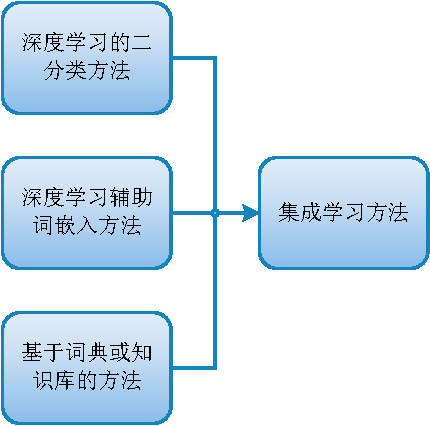
\includegraphics{overall}
	\caption{四种研究方法间的关系}
	\label{f:overall}
	\vspace{-1em}
\end{figure}

\BiSubsection{深度学习的二分类方法}{}
将困难问题规约到简单问题是科学研究中常用的手法,本方法将词语相似度计算这一无监督回归问题转化为有监督分类问题,以降低解决问题的难度。对于句子的分类问题,本方法使用循环神经网络以及它们的变种 LSTM 予以解决。

\BiSubsection{深度学习辅助词嵌入方法}{}
词嵌入是自然语言处理中的一项非常成熟的技术,它可以将词语映射到向量空间中。而向量具有天然的相似度评价方法,这使得词嵌入技术经常被用于解决词语相似度计算问题。本方法查找现有词嵌入技术中的局限性,并使用深度学习方法拓展现有词嵌入技术,以改善它们的性能。

\BiSubsection{基于词典或知识库的方法}{}
很多现有的语言学资料中提供了对词语语义的一些形式化的解释。这些解释可以被计算机解析和利用,因此也可以作为词语相似度计算的素材。本方法尝试使用现有的词典或知识库资源,并对业界常用的利用它们进行词语相似度计算的方法进行一些改进。

\BiSubsection{集成学习方法}{}
实际的词语相似度计算系统多是多种方法的结合。这有助于发挥各方法的长处,同时提高系统的稳定性。在其它开放任务参赛队发表的系统中,集成多种技术最常见的方法是简单平均法和加权平均法。除此之外,很多人为制定的基于规则的结合策略也被用于此用途。这些方法虽然简单朴素,甚至有些看起来缺乏理论根据,但是在词语相似度计算的任务中取得了相当优秀的成绩。尽管如此,发现一个好的结合规则仍然需要大量实验和一定的运气成分。因此,需要借助集成学习的技术来发现一种更可靠的、表现更为稳定的方法。